\documentclass[10pt,journal,compsoc,onecolumn]{IEEEtran}
\usepackage{amsmath,amsfonts,amssymb}
\usepackage{mathtools}
\usepackage{algorithm}
\usepackage{array}
\usepackage[caption=false,font=normalsize,labelfont=sf,textfont=sf]{subfig}
\usepackage{textcomp}
\usepackage{stfloats}
\usepackage{url}
\usepackage{verbatim}
\usepackage{graphicx}
\ifCLASSOPTIONcompsoc
  \usepackage[nocompress]{cite}
\else
  \usepackage{cite}
\fi
\usepackage{booktabs}
\usepackage{graphicx}
\usepackage{enumitem}
\usepackage{multirow}
\usepackage{pifont}
\usepackage{makecell}
\usepackage{tabularx}
\usepackage{algpseudocode}
\usepackage{tikz}
\usetikzlibrary{positioning,arrows.meta}
\usepackage[strings]{underscore}
\usepackage{hyperref}
\usepackage{cleveref}
\usepackage[dvipsnames]{xcolor}
\hypersetup{hidelinks}
\setcounter{secnumdepth}{3}
\hyphenation{op-tical net-works semi-conduc-tor IEEE-Xplore}
% updated with editorial comments 8/9/2021

\begin{document}

\title{DeXposure-Agent: An Agentic System for DeFi Risk Monitor and Decision based on Graph Times-Series Foundation Model}

\author{Aijie~Shu and Fengxiang~He%
\IEEEcompsocitemizethanks{%
\IEEEcompsocthanksitem A. Shu and F. He are with the School of Informatics, University of Edinburgh, Edinburgh EH8 9AB, U.K. (e-mail: v1ashu@ed.ac.uk; F.He@ed.ac.uk).
\IEEEcompsocthanksitem Corresponding author: Fengxiang He.}}%
%\thanks{Manuscript received April 19, 2021; revised August 16, 2021.}}

\markboth{IEEE Transactions on Knowledge and Data Engineering}%
{Shu and He: DeXposure-Agent}

% The paper headers
%\markboth{Journal of \LaTeX\ Class Files,~Vol.~14, No.~8, August~2021}%{Shell \MakeLowercase{\textit{et al.}}: A Sample Article Using IEEEtran.cls for IEEE Journals}

%\IEEEpubid{0000--0000/00\$00.00~\copyright~2021 IEEE}
% Remember, if you use this you must call \IEEEpubidadjcol in the second
% column for its text to clear the IEEEpubid mark.

\IEEEtitleabstractindextext{%
\begin{abstract}
Decentralised finance (DeFi) has become a densely interconnected financial system in which credit exposures propagate through tokenised liabilities across protocols, making timely \emph{risk monitoring} and \emph{decision recommendation} essential for investors, protocol operators, and regulators. Existing agentic pipelines for DeFi risk lack a dedicated forecasting backbone for graph-structured time series, which limits their data efficiency and uncertainty calibration. Building on DeXposure-FM, a graph time-series foundation model pre-trained on $43.7$ million exposure-graph entries, we present two contributions. First, \emph{DeXposure-Framework}: a four-layer query architecture---FM prediction, deterministic monitoring and scenario, LLM decision, and a data-health/confidence safety gate---that turns predicted exposure graphs into supervisory tickets. Second, \emph{DeXposure-Bench}: a six-axis evaluation suite for FM\,+\,LLM decision pipelines on temporal exposure graphs, with a regulator-aligned ground truth defined by absolute exposure loss. The bench surfaces a non-trivial Pareto trade-off rather than uniform improvement: persistence remains strong on point-metric forecasting and ticket precision, while the FM turns forecasting into a deployable risk signal through trend consistency, calibrated uncertainty (PI coverage $0.912$ against a $0.90$ target), and robustness. In layer-wise decision ablations, the FM and LLM layers make additive contributions to ticket F1 ($+32\%$ from FM and $+27\%$ from LLM), while the safety gate improves explanation quality at a small F1 cost. We release the harness, dataset, and reference implementations to support extension.

Code: \href{https://github.com/EVIEHub/DeXposure-Agent}{https://github.com/EVIEHub/DeXposure-Agent}

Demo: \href{https://www.youtube.com/}{https://www.youtube.com/}
\end{abstract}

\begin{IEEEkeywords}
Agentic system, graph, time series, foundation model, decentralised finance, financial network, risk modelling.
\end{IEEEkeywords}}

\maketitle
\IEEEdisplaynontitleabstractindextext
\IEEEpeerreviewmaketitle

\section{Introduction}
\label{sec:introduction}

Decentralised finance (DeFi) has rapidly evolved into a densely interconnected financial system in which protocols are linked through tokenised liabilities, rehypothecation, wrapping, bridging, and composable yield strategies. These linkages form an evolving \emph{credit-exposure network}: shocks to one protocol (e.g., insolvency, de-pegging, oracle failures, liquidity runs, or governance attacks) can propagate through downstream balance sheets and induce systemic stress. In such a setting, timely \emph{risk monitoring} and \emph{decision recommendation} are essential for investors, protocol operators, and regulators. Yet DeFi risk management remains challenging in practice: exposures are high-dimensional, time-varying, and often implicit; data are noisy and incomplete; and crises unfold quickly, leaving limited time for manual assessment.

A natural response is to build \emph{agentic} pipelines that automate surveillance and intervention planning. In principle, an agent can ingest on-chain measurements, maintain a belief over the evolving exposure network, surface early-warning signals, stress-test plausible shocks, and recommend risk-mitigating actions with auditable rationale. However, despite growing interest, agentic DeFi risk systems remain premature. A core bottleneck is the lack of a reliable \emph{foundation model backbone} for dynamic exposure networks: without accurate and data-efficient forecasting of graph time-series dynamics, monitoring agents are prone to false alarms and delayed detection, while decision agents risk recommending actions based on brittle or poorly calibrated beliefs. Unlike many recent multi-agent proposals that glue together large language models or other massive neural networks, our pipeline does not depend on such general-purpose big models; instead it uses a specialised graph–time‑series backbone tailored to the problem domain. In high-stakes contexts, uncertainty calibration and robustness to missingness and regime shifts are not optional - they determine whether an agent is trusted and deployable.

This paper addresses that bottleneck by building an agentic system around a strong graph time-series foundation model. We leverage DeXposure-FM, a recent foundation model trained on over $43.7$ million data entries, designed to forecast the evolution of DeFi exposure networks in a multi-horizon setting. On top of this predictive backbone, we develop \emph{DeXposure-Agent}, which, to our best knowledge, is the first agentic system for DeFi risk monitoring and decision recommendation. The system instantiates a conservative but operationally meaningful loop: it continuously ingests exposure snapshots, uses {DeXposure-FM} to forecast future credit-exposure graphs, computes systemic risk indicators and standardised stress scenarios, and emits auditable alerts and playbook-based recommendations under explicit data-health and uncertainty gates. The design is intentionally modular: the foundation model provides probabilistic forecasts; the monitoring layer translates forecasts into interpretable risk signals; the scenario engine evaluates stress outcomes; and the decision layer maps signals into recommendations while enforcing guardrails for safe deployment.

%\paragraph{DeXposure-Agent overview.}
DeXposure-Agent follows a \emph{forecast-measure-decision} paradigm. At each epoch, it (1) checks the integrity of the incoming graph snapshot via a data-health gate, (2) forecasts multi-step future exposure networks using {DeXposure-FM}, (3) computes risk measurements on predicted graphs (e.g., concentration, spillovers, and systemic importance) and evaluates a standardised library of stress scenarios, and (4) outputs a ranked set of alerts and decision tickets. Each alert is accompanied by evidence (triggering metric deviations), attribution (top contributing nodes/edges/sectors), and uncertainty-aware confidence. Each decision ticket is conservative and auditable: it links back to explicit triggers, includes scenario-based impact summaries, and is suppressed or downgraded when data quality or model reliability degrades. This design reflects a key principle: in DeFi risk management, the ability to say \emph{``we do not know''} is as important as the ability to recommend an action.

To make this pipeline concrete we implemented a modular architecture. on-chain TVL/token data are pulled from public APIs such as DefiLlama, transformed through a token–protocol mapping and assembled into discrete exposure graph snapshots; a lightweight data-health service scores each snapshot and triggers a safe mode when needed. The prediction backbone runs as a separate inference service—the DeXposure‑FM model returns probability distributions over future graphs along multiple horizons, supporting both expected‑weight construction and Monte Carlo sampling. A monitoring layer computes a set of systemic indices on the representative forecast, maintains rolling baselines for triggers, attributes alerts by marginal contribution, and quantifies forecast uncertainty. A parallel scenario engine applies a library of standardised shocks to the same forecasts and ranks outcomes by expected/tail loss. Finally a decision module consults a small playbook of conservative actions, enforces data‑health and confidence gates, scores and ranks tickets, and exposes results via an API and dashboard. All components communicate through simple data structures, so the system can be deployed as microservices or as a single Python application depending on operational needs.

%\paragraph{Evaluation and findings.}
We evaluate DeXposure-Agent across xx benchmarks and stress-test settings, including low-data and weakly supervised regimes that reflect real operational constraints. We compare against state-of-the-art methods for spatio-temporal/graph risk forecasting and against agentic baselines that do not leverage a dedicated graph time-series foundation model backbone. The results show that DeXposure-Agent: (1) produces earlier and more stable early-warning signals of systemic fragility,
(2) improves risk metric forecasting and uncertainty calibration, and
(3) yields higher-quality recommendation tickets (more robust, better justified, and less sensitive to noise),
all significantly outperforming existing approaches in both predictive accuracy and operational utility.
An open-source implementation is available at
\href{https://github.com/EVIEHub/DeXposure-Agent}{https://github.com/EVIEHub/DeXposure-Agent}.
\section{Related Works}

This section surveys prior work most closely related to our setting.

\subsection{Financial Network Risk Modelling}
In traditional finance, credit risk modelling typically spans both entity-level default modelling and system-level network perspectives. Classical structural and reduced-form approaches focus on estimating default likelihoods for individual institutions, whereas network contagion models study how distress can cascade through interconnected balance sheets. For instance, Dolfin et al. use network epidemic models to study credit contagion, showing that dense interconnections and overlapping portfolios can magnify systemic credit risk \cite{math7080713}.

In decentralised finance, credit risk takes a different form because lending is commonly over-collateralised and enforced by smart contracts. Bertomeu et al. introduce parsimonious aggregate risk measures for DeFi lending protocols based only on total deposits and borrowings, and find that systemic fragility rose sharply around mid-2021 during periods of crypto-market stress \cite{BERTOMEU2024105321}. Bridging conceptual links between TradFi and DeFi, Aufiero et al. review mechanisms of systemic risk and argue that, while familiar ingredients (leverage, liquidity shocks, correlated exposures) exist in both systems, DeFi’s algorithmic execution and composability introduce distinctive channels through which shocks may propagate \cite{aufiero2025mappingmicroscopicsystemicrisks}.

\subsection{Machine Learning Approaches}

Machine learning methods are increasingly used for systemic-risk detection and contagion analysis \cite{BALMASEDA2023200240, gonon2025computingsystemicriskmeasures}. In particular, graph neural networks (GNNs) exploit relational structure to strengthen predictive performance on networked risk problems \cite{KipfWelling2017, veličković2018graphattentionnetworks}. Balmaseda et al. demonstrate that GNN-based models can substantially outperform conventional ML when classifying the systemic importance of banks in simulated financial networks \cite{BALMASEDA2023200240}. Gonon et al. combine GNNs with explicit interbank liability networks to compute systemic risk measures defined via the minimum capital required to stabilise the system \cite{gonon2025computingsystemicriskmeasures}. Their formulation effectively captures contagion channels (e.g., Eisenberg--Noe-style clearing) by embedding graph-structured information directly into the risk aggregation procedure.

\subsection{Foundation Models}

Foundation models are increasingly influencing finance and economics by shifting from narrowly tuned, task-specific models towards reusable representations learned from broad data. Rather than training a bespoke model per downstream objective, recent work pretrains large neural networks---predominantly transformer-based architectures \cite{VaswaniEtAl2017Attention} and related variants---on massive corpora, then transfers these models across tasks via prompting or lightweight adaptation \cite{AnsariEtAl2024Chronos,RasulEtAl2023LagLlama,DasEtAl2024TimesFM}. Alongside this, an emerging policy-oriented literature uses large language models to extract quantitative signals from narrative sources (e.g., reports, releases, and news) and to integrate them into nowcasting pipelines, suggesting that relatively small yet information-rich text inputs can improve real-time forecasting when paired with standard indicators \cite{deBondtSun2025ChatGPTNowcast,KwonEtAl2024BISLLMprimer,CarrieroEtAl2024MacroLLM}. 

Foundation-model ideas are also being extended to graph-structured inputs by augmenting self-attention with graph-aware structural encodings, illustrating the viability of large pretrained models for networks that resemble webs of financial contracts or cross-asset relationships; Graphormer provides a representative example \cite{Ying2021Graphormer}. For tabular settings, the Graph Prior-data Fitted Network (GraphPFN) \cite{eremeev2025turningtabularfoundationmodels} is pretrained on millions of synthetic tabular tasks and reports strong out-of-the-box performance across a range of benchmarks.
\section{Notation and Preliminaries}

This section introduces the key terminology and notation used throughout the paper.

\subsection{Credit Exposure in DeFi Networks}

Let $X_G(q)$ be the set of tokens issued (or generated) by protocol $q$, and let $X_p(t)$ be the set of tokens held (or locked) by protocol $p$ at time $t$. We say that protocol $p$ has \emph{credit exposure} to protocol $q$ at time~$t$ if $p$ holds at least one token issued by $q$:
\begin{equation}
X_p(t)\cap X_G(q)\neq \varnothing.
\label{eq:credit-exposure-definition}
\end{equation}
Equivalently, $p$ is exposed to liabilities of $q$: if tokens issued by $q$ devalue or become illiquid, $p$ incurs losses. This token-mediated dependence generalises counterparty credit risk from traditional finance to DeFi, where exposures emerge through tokenised claims rather than explicit bilateral contracts. In practice, these dynamics can be tracked by reconstructing protocol-level TVL time series and monitoring how token composition changes over time \cite{wu2025dexposuredatasetbenchmarksinterprotocol}.

Figure~\ref{fig:exposure_example} shows how a single workflow can generate layered exposures. A user deposits ETH into Lido and receives stETH; stETH is wrapped into wstETH; wstETH is then deposited into Pendle, which splits it into PT-wstETH and YT-wstETH. On balance sheets, each step turns the upstream token into the downstream protocol's asset, so exposures stack: Pendle is exposed to the wstETH wrapper, which is exposed to Lido. If Lido suffers slashing or stETH de-pegs from ETH, losses can propagate through wstETH into Pendle and its PT/YT holders. This illustrates why DeFi exposures are naturally multi-layered and why DeXposure aims to measure them.

\begin{figure}[t]
    \centering
    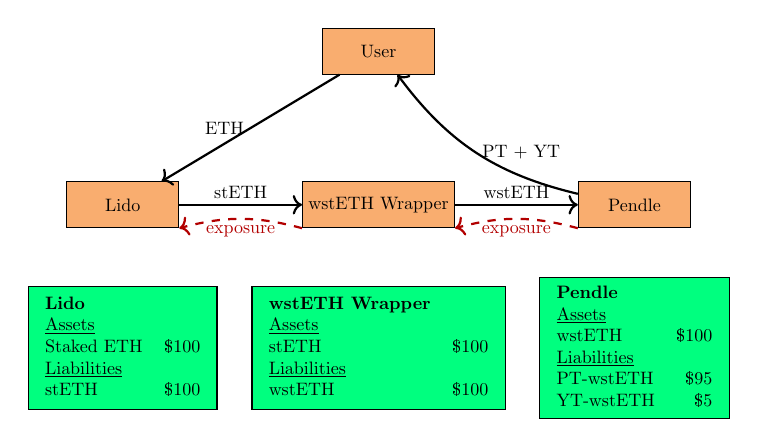
\begin{tikzpicture}[node distance=1.8cm, auto, scale=0.65, transform shape]
        \tikzstyle{entity} = [rectangle, draw, fill=Apricot, minimum width=2.2cm, minimum height=0.9cm, font=\normalsize]
        \tikzstyle{balance} = [rectangle, draw, fill=SpringGreen, minimum width=3.2cm, minimum height=2.4cm, font=\normalsize]
        \tikzstyle{exposure} = [->, thick, dashed, red!70!black]

        % User at top
        \node[entity] (user) at (0,3) {User};

        % Three protocols in a row
        \node[entity] (lido) at (-5,0) {Lido};
        \node[entity] (wrapper) at (0,0) {wstETH Wrapper};
        \node[entity] (pendle) at (5,0) {Pendle};

        % Balance sheets below each protocol
        \node[balance] (balanceLido) at (-5,-2.8) {
            \begin{tabular}{lr}
                \textbf{Lido} & \\
                \underline{Assets} & \\
                Staked ETH & \$100 \\
                \underline{Liabilities} & \\
                stETH & \$100
            \end{tabular}
        };
        \node[balance] (balanceWrapper) at (0,-2.8) {
            \begin{tabular}{lr}
                \textbf{wstETH Wrapper} & \\
                \underline{Assets} & \\
                stETH & \$100 \\
                \underline{Liabilities} & \\
                wstETH & \$100
            \end{tabular}
        };
        \node[balance] (balancePendle) at (5,-2.8) {
            \begin{tabular}{lr}
                \textbf{Pendle} & \\
                \underline{Assets} & \\
                wstETH & \$100 \\
                \underline{Liabilities} & \\
                PT-wstETH & \$95 \\
                YT-wstETH & \$5
            \end{tabular}
        };

        % Token flows (solid arrows)
        \draw[->, thick] (user) -- node[left, font=\normalsize] {ETH} (lido);
        \draw[->, thick] (lido) -- node[above, font=\normalsize] {stETH} (wrapper);
        \draw[->, thick] (wrapper) -- node[above, font=\normalsize] {wstETH} (pendle);
        \draw[->, thick] (pendle) to[bend left=20] node[right, font=\normalsize] {PT + YT} (user);

        % Credit exposure arrows (dashed red)
        \draw[exposure] (pendle.south west) to[bend right=15] node[below, font=\normalsize, text=red!70!black] {exposure} (wrapper.south east);
        \draw[exposure] (wrapper.south west) to[bend right=15] node[below, font=\normalsize, text=red!70!black] {exposure} (lido.south east);

    \end{tikzpicture}
    \caption{Multi-layer credit exposure in DeFi. A user stakes ETH with Lido, receiving stETH, which is wrapped into wstETH and deposited into Pendle. Each protocol holds the liability of the preceding one, creating a chain of credit exposures from Pendle to Lido.}
    \label{fig:exposure_example}
\end{figure}

\subsection{Mapping Tokens to Issuing Protocols}

To implement Eq.~\eqref{eq:credit-exposure-definition}, we must identify the issuing (or managing) protocol for each token. Let $\mathcal{P}$ be the set of protocols and $\mathcal{C}$ the set of blockchains. For any token $\sigma$ appearing in protocol $p$, a \emph{mapping function} $M(\sigma)$ returns the protocol $q$ that issues or governs $\sigma$. We construct $M$ via the following fallback pipeline:
\begin{enumerate}
  \item \emph{Metadata lookup:} match tokens to issuing protocols using DefiLlama metadata when available \cite{DefiLlama2026}.
  \item \emph{Manual mapping:} for high-TVL tokens without metadata links, assign issuers using documentation and expert judgment.
  \item \emph{Text-vector similarity:} otherwise, vectorise token and protocol descriptions using TF-IDF \cite{Qaiser2018} and assign $M(\sigma)$ as the most similar protocol, provided the cosine similarity exceeds a threshold $\theta$.
  \item \emph{Primary market tokens:} if no match is obtained, treat the token as its own protocol (e.g., WETH).
\end{enumerate}
This procedure attributes token movements to the appropriate issuer even when tokens are bridged or wrapped, and is used in curating DeXposure.

\subsection{Network Representation and Value Flows}

Over a discrete interval $\tau=t_2-t_1$, we represent exposures by a weighted directed graph $G_\tau=(P_\tau,E_\tau)$, where $P_\tau$ is the set of active protocols and $E_\tau$ the directed edge set. Each node $p\in P_\tau$ receives a \emph{node weight} equal to the value of its held assets at $t_2$:
\begin{equation}
w_\tau(p) = \sum_{\sigma\in X_p(t_1)\cap X_p(t_2)} v_{t_2,\sigma},
\label{eq:node-weight}
\end{equation}
where $v_{t_2,\sigma}$ is the USD value of token $\sigma$ at time $t_2$. Nodes below a threshold $\theta$ may be pruned.

To define the \emph{edge weight} from $p$ to $q$, we first compute token-level value flows:
\begin{equation}
F^{\sigma}_{p q,\tau} =
\begin{cases}
\max\bigl(0,\, -\Delta S^{\sigma}_{p,\tau}\bigr), & \text{if } \Delta S^{\sigma}_{p,\tau} < 0,\\
\max\bigl(0,\,\Delta S^{\sigma}_{q,\tau}\bigr), & \text{if } \Delta S^{\sigma}_{q,\tau} \ge 0,
\end{cases}
\label{eq:value-flow}
\end{equation}
where $\Delta S^{\sigma}_{p,\tau}=v_{p,t_2}^{\sigma}-v_{p,t_1}^{\sigma}$ is the change in the USD value of token $\sigma$ held by $p$ over $\tau$. Intuitively, if $p$ reduces holdings while $q$ increases holdings, $\sigma$ is interpreted as flowing from $p$ to $q$; the construction enforces non-negativity.

The \emph{edge weight} $w_\tau(e_{p q})$ aggregates flows over tokens mapped to issuer $q$:
\begin{equation}
w_\tau(e_{p q}) = \sum_{\sigma \in X_{p q, \tau}} F^{\sigma}_{p q,\tau},
\label{eq:edge-weight}
\end{equation}
where $X_{p q,\tau}$ is the set of tokens issued by $q$ that move from $p$ to $q$ over $\tau$. Positive $w_\tau(e_{p q})$ corresponds to increasing exposure from $p$ to $q$; for single-token protocols, that token's flow equals the edge weight. In summary, we compute $G_\tau$ by aggregating holdings at $t_1$ and $t_2$, assigning node weights, pruning small nodes, and summing positive token flows into issuer-specific edge weights. The resulting graph sequence captures the evolving credit-dependency structure curated in DeXposure.

\section{Algorithm}
\label{sec:algorithm}

This section specifies the agentic system built on \textsc{DeXposure-FM} for two tasks: monitoring and decision-making. 

\subsection{Task I: Network Risk Monitoring}
\label{subsec:task_monitoring}

At each decision epoch $t$, we observe a current DeFi credit-exposure snapshot $G_t=(V,E_t,W_t)$ and node covariates $X_t$ (e.g., log-TVL and auxiliary features). Given a set of forecast horizons $\mathcal{H}$, the foundation model \textsc{DeXposure-FM} induces predictive distributions over future exposure networks,
\begin{equation}
\mathcal{P}_{t,h} \;:=\; p\!\left(G_{t+h}\mid G_{\le t}, X_{\le t}\right), \qquad h\in\mathcal{H}.
\end{equation}
We denote by $\widehat{G}_{t+h}$ a representative predicted network constructed from $\mathcal{P}_{t,h}$ (e.g., the expected-weight graph), and by $\widetilde{G}^{(m)}_{t+h}\sim\mathcal{P}_{t,h}$ a sampled predicted network for uncertainty quantification.

\paragraph{Monitoring objective.}
The monitoring agent computes a collection of systemic indicators (``measurements'') as functionals of predicted networks:
\begin{equation}
\mathbf{M}_{t,h} \;:=\; \Phi\!\left(\widehat{G}_{t+h}, X_t\right)\in\mathbb{R}^d,
\qquad
\widetilde{\mathbf{M}}^{(m)}_{t,h} \;:=\; \Phi\!\left(\widetilde{G}^{(m)}_{t+h}, X_t\right),
\end{equation}
where $\Phi$ may include, for example, concentration indices, sector spillover measures, systemic importance scores, and stress-test losses. Let $\mathcal{B}_t(\cdot)$ be a baseline band operator derived from historical measurements (e.g., rolling mean and standard deviation). The monitoring agent issues an alert when a predicted measurement departs from its baseline beyond a tolerance:
\begin{equation}
\label{eq:monitor_alert_rule}
\mathcal{A}_t \;:=\; \Bigl\{\, a=(h,j): \; g\!\left(M_{t,h}^{(j)}, \mathcal{B}_t^{(j)}\right)=1 \Bigr\},
\end{equation}
where $M_{t,h}^{(j)}$ is the $j$-th component of $\mathbf{M}_{t,h}$, $\mathcal{B}_t^{(j)}$ is the corresponding baseline band, and $g(\cdot)$ is a trigger rule (e.g., a $z$-score or change-point test). 

\paragraph{Uncertainty-aware confidence.}
To expose forecast uncertainty, the agent attaches an alert confidence score. Let $\mathrm{U}_{t,h}^{(j)}$ denote a dispersion statistic (e.g., inter-quantile range) computed from $\{\widetilde{\mathbf{M}}^{(m)}_{t,h}\}_{m=1}^M$, and let $DH_t\in[0,1]$ be a data-health score. We define a generic confidence mapping
\begin{equation}
\label{eq:monitor_confidence}
C_t(a)\;=\;\psi\!\left(DH_t,\, \mathrm{U}_{t,h}^{(j)},\, h\right)\in[0,1],
\end{equation}
so alerts carry both evidence (triggering statistics) and reliability (data/model quality).


\subsection{Task II: Decision-Making}
\label{subsec:task_decision}

The decision-making agent consumes monitoring alerts $\mathcal{A}_t$ and predictive distributions $\{\mathcal{P}_{t,h}\}_{h\in\mathcal{H}}$ to propose risk-mitigating actions. Let $\mathcal{U}$ denote a feasible action set (e.g., watchlist updates, exposure reduction recommendations, governance parameter suggestions). An action $u\in\mathcal{U}$ induces an intervention operator on the current state,
\begin{equation}
T(u): (G_t, X_t)\mapsto (G_t^{u}, X_t^{u}),
\end{equation}
representing, for example, reduced exposure to certain protocols, altered risk limits, or scenario-dependent constraints. Under $u$, the foundation model yields counterfactual predictive distributions
\begin{equation}
\mathcal{P}^{u}_{t,h} \;:=\; p\!\left(G_{t+h}\mid G_{\le t}^{u}, X_{\le t}^{u}\right), \qquad h\in\mathcal{H}.
\end{equation}
Let $\mathcal{S}$ be a library of standardised stress scenarios (shocks) applied to predicted networks, and let $\ell(\cdot)$ be a nonnegative systemic loss functional (e.g., stress-test loss, tail concentration, spillover loss). For a scenario $s\in\mathcal{S}$, define the (random) loss at horizon $h$:
\begin{equation}
L_{t,h}(u,s) \;:=\; \ell\!\left(G_{t+h}^{u,s}\right), \qquad
G_{t+h}^{u,s} \sim \mathcal{P}^{u}_{t,h}\ \text{with scenario } s,
\end{equation}
and an uncertainty-aware risk aggregation (e.g., expectation plus tail risk):
\begin{equation}
\label{eq:risk_objective}
\mathcal{R}_t(u) \;:=\; \sum_{h\in\mathcal{H}} \omega_h \cdot 
\max_{s\in\mathcal{S}} \Bigl(
\mathbb{E}[L_{t,h}(u,s)] + \lambda\cdot \mathrm{CVaR}_{\alpha}(L_{t,h}(u,s))
\Bigr),
\end{equation}
where $\omega_h$ are horizon weights, $\lambda\ge 0$ controls tail sensitivity, and $\alpha\in(0,1)$ is a tail level.

\paragraph{Decision objective with constraints.}
Let $\mathrm{cost}(u)$ be the operational cost of recommending or implementing $u$ (including conservativeness penalties), and let $\mathcal{C}_t$ encode safety constraints such as data-health and calibration gates. The decision-making task is to select a recommendation
\begin{equation}
\label{eq:decision_problem}
u_t^\star \;\in\; \arg\min_{u\in\mathcal{U}} \ \mathcal{R}_t(u) + \eta\cdot \mathrm{cost}(u)
\quad \text{s.t.}\quad u \in \mathcal{C}_t,
\end{equation}
where $\eta\ge 0$ trades off risk reduction and operational cost. In the minimal viable agent, $\mathcal{U}$ is restricted to a small set of conservative playbooks and $\mathcal{C}_t$ enforces strict gating: when $DH_t$ (or calibration) is low, the feasible set collapses to non-interventional actions (e.g., \texttt{Monitor}/\texttt{Investigate} recommendations).

\paragraph{Decision outputs.}
The agent returns a ranked set of recommendation tickets $\mathcal{D}_t=\{(u,r(u))\}$, each with (i) the proposed action $u$, (ii) an estimated risk reduction $r(u)$ derived from \eqref{eq:risk_objective}--\eqref{eq:decision_problem}, and (iii) an evidence bundle summarizing the triggering alerts, scenario impacts, and uncertainty measures.

\subsection{System Interface}
At each epoch $t$, the agent receives the latest state (graph snapshot and features) and returns: (a) a set of monitoring alerts with evidence and confidence, (b) a scenario stress summary, and (c) a ranked list of recommendation tickets. The agent interacts with \textsc{DeXposure-FM} through a single primitive:
\begin{equation}
\label{eq:agent_forecast_primitive}
\mathcal{P}_{t,h} \leftarrow \textsc{DeXposure-FM}.\mathrm{Forecast}(G_t,X_t,h), \forall h\in\mathcal{H},
\end{equation}
where $\mathcal{P}_{t,h}$ denotes the model's predictive distribution for horizon $h$. We use a deterministic graph-construction operator $\mathrm{BuildPredGraph}(\cdot)$ to obtain a representative forecasted network $\widehat{G}_{t+h}$ from $\mathcal{P}_{t,h}$ (e.g., expected-weight or thresholded-probability construction). Optionally, we draw Monte Carlo samples $\{\widetilde{G}^{(m)}_{t+h}\}_{m=1}^M$ for uncertainty quantification.

\subsection{Data-Health Gating}
\label{subsec:data_health_gate}
Before producing actionable outputs, the agent computes a scalar data-health score
\begin{align}
\label{eq:data_health}
&DH_t \leftarrow \mathrm{DataHealth}(G_t,X_t)\in[0,1],\nonumber\\
&\mathrm{SAFE\_MODE}_t := \mathbb{I}\{DH_t<\tau_{\mathrm{data}}\}.
\end{align}
$\mathrm{DataHealth}(\cdot)$ aggregates deterministic checks including freshness, missingness, discontinuities/outliers, and topology sanity. In safe mode, the agent still emits monitoring alerts but suppresses intervention-type recommendations (Section~\ref{subsec:decision_v1}).

\subsection{Monitoring: Forecast--then--Measure--then--Alert}
\label{subsec:monitoring_agent}
For each horizon $h\in\mathcal{H}$, the agent forecasts $\mathcal{P}_{t,h}$ by \eqref{eq:agent_forecast_primitive}, constructs $\widehat{G}_{t+h}$, and evaluates a vector of monitoring functionals:
\begin{equation}
\label{eq:monitor_metrics}
\mathbf{M}_{t,h} := \Phi(\widehat{G}_{t+h},X_t)\in\mathbb{R}^d,~
\widetilde{\mathbf{M}}^{(m)}_{t,h} := \Phi(\widetilde{G}^{(m)}_{t+h},X_t),
\end{equation}
where $\Phi(\cdot)$ includes the systemic indicators used by the monitoring dashboard (e.g., systemic-importance ranking, cross-sector spillover concentration, stability/concentration indices, and stress-test losses). Let $\mathcal{B}_t^{(j)}$ be a baseline band for the $j$-th metric (e.g., a rolling mean/standard deviation band over a fixed historical window). An alert is triggered when a forecasted metric departs from its baseline:
\begin{equation}
\label{eq:alert_trigger_generic}
\mathcal{A}_t :=
\Bigl\{\, a=(h,j)\;:\; g\!\bigl(M_{t,h}^{(j)},\,\mathcal{B}_t^{(j)}\bigr)=1 \Bigr\},
\end{equation}
where $g(\cdot)$ is a deterministic trigger (e.g., $z$-score, change-point score, or rule-based condition).

\paragraph{Evidence and attribution.}
Each alert $a=(h,j)\in\mathcal{A}_t$ is returned with an evidence bundle:
\begin{equation}
\label{eq:alert_evidence}
\mathrm{Ev}_t(a) := \Bigl( M_{t,h}^{(j)},\ \mathcal{B}_t^{(j)},\ \mathrm{Attr}_t(a),\ h \Bigr),
\end{equation}
where $\mathrm{Attr}_t(a)$ denotes a ranked set of contributing nodes/edges/sectors obtained via marginal contribution approximations on the corresponding functional $\Phi^{(j)}(\cdot)$.

\paragraph{Uncertainty-aware confidence.}
Using sampled metric realizations $\{\widetilde{\mathbf{M}}^{(m)}_{t,h}\}_{m=1}^M$, we compute a dispersion statistic $\mathrm{U}_{t,h}^{(j)}$ (e.g., inter-quantile range) and attach a confidence score:
\begin{equation}
\label{eq:alert_confidence_generic}
C_t(a) := \psi\!\left(DH_t,\ \mathrm{U}_{t,h}^{(j)},\ h\right)\in[0,1],
\end{equation}
which monotonically decreases with lower data health, wider predictive spread, and longer horizons.

\subsection{Scenario Engine}
\label{subsec:scenario_engine}
To support systematic triage, the agent evaluates a small standardised scenario set $\mathcal{S}_0$ (stress shocks). For each horizon $h$ and scenario $s$, we compute a scenario loss functional:
\begin{equation}
\label{eq:scenario_loss}
L_{t,h}(s) := \ell\!\left(\widehat{G}_{t+h}; s\right),~
\widetilde{L}^{(m)}_{t,h}(s) := \ell\!\left(\widetilde{G}^{(m)}_{t+h}; s\right),
\end{equation}
where $\ell(\cdot;\,s)$ denotes the stress-test procedure applied to the predicted network under shock $s$. The scenario summary $\mathcal{R}_t$ ranks scenarios by expected (or median) loss and highlights worst-case horizons and dominant propagation channels via the same attribution interface used in monitoring.

\subsection{Decision Agent v1: Conservative Playbook Recommendations}
\label{subsec:decision_v1}
The decision module maps $(\mathcal{A}_t,\{\mathrm{Ev}_t(a),C_t(a)\},\mathcal{R}_t)$ to a ranked set of recommendation tickets. Let $\mathcal{U}$ be a set of conservative recommendation types (e.g., watchlist update, escalated monitoring, investigation request, exposure reduction suggestion, contingency planning). Each $u\in\mathcal{U}$ must satisfy a safety constraint set $\mathcal{C}_t$:
\begin{align}
\label{eq:decision_constraints}
&u \in \mathcal{C}_t
\quad \Longleftrightarrow \nonumber\\
&\Bigl(\mathrm{SAFE\_MODE}_t=0\Bigr)\ \wedge\ \Bigl(\min_{a\in \mathrm{Trig}(u)} C_t(a) \ge \tau_{\mathrm{conf}}\Bigr),
\end{align}
where $\mathrm{Trig}(u)\subseteq\mathcal{A}_t$ denotes the subset of alerts required to justify $u$. In safe mode, the feasible set collapses to non-interventional actions (e.g., \texttt{Monitor}/\texttt{Investigate}).

\paragraph{Ticket ranking.}
Each feasible recommendation is scored by a monotone heuristic combining severity, confidence, and scenario impact:
\begin{equation}
\label{eq:ticket_score}
\mathrm{Score}_t(u) :=
\mathrm{Sev}_t(u)\cdot \mathrm{Conf}_t(u)\cdot \mathrm{Imp}_t(u),
\end{equation}
where $\mathrm{Sev}_t(u)$ is derived from triggered metric deviations, $\mathrm{Conf}_t(u)$ aggregates $C_t(a)$ over required alerts, and $\mathrm{Imp}_t(u)$ is derived from $\mathcal{R}_t$ (e.g., worst-case scenario loss). The decision agent returns a ranked ticket list $\mathcal{D}_t=\{(u,\mathrm{Score}_t(u),\mathrm{Ev}_t(u))\}$, where $\mathrm{Ev}_t(u)$ bundles alert evidence, scenario summaries, and an auditable rationale.

\subsection{End-to-End Procedure}
Algorithm~\ref{alg:agent_loop} summarises the minimal viable agent loop.

\begin{algorithm}[t]
\caption{DeXposure-Agent}
\label{alg:agent_loop}
\begin{algorithmic}[1]
\Require Current state $(G_t,X_t)$; horizons $\mathcal{H}$; scenarios $\mathcal{S}_0$; baseline bands $\{\mathcal{B}_t^{(j)}\}_{j=1}^d$; thresholds $(\tau_{\mathrm{data}},\tau_{\mathrm{conf}})$
\Ensure Alerts $\mathcal{A}_t$ with evidence/confidence; scenario summary $\mathcal{R}_t$; recommendation tickets $\mathcal{D}_t$
\State $DH_t \gets \mathrm{DataHealth}(G_t,X_t)$; $\mathrm{SAFE\_MODE}_t \gets \mathbb{I}\{DH_t<\tau_{\mathrm{data}}\}$
\ForAll{$h\in\mathcal{H}$}
    \State $\mathcal{P}_{t,h} \gets \textsc{DeXposure-FM}.\mathrm{Forecast}(G_t,X_t,h)$
    \State $\widehat{G}_{t+h} \gets \mathrm{BuildPredGraph}(\mathcal{P}_{t,h})$
    \State $\mathbf{M}_{t,h} \gets \Phi(\widehat{G}_{t+h},X_t)$
    \State $\mathcal{A}_{t,h} \gets \{(h,j): g(M^{(j)}_{t,h},\mathcal{B}_t^{(j)})=1\}$
    \State attach $\mathrm{Ev}_t(a)$ and $C_t(a)$ for all $a\in\mathcal{A}_{t,h}$
    \State compute scenario losses $\{L_{t,h}(s)\}_{s\in\mathcal{S}_0}$ and attributions
\EndFor
\State $\mathcal{A}_t \gets \bigcup_{h\in\mathcal{H}}\mathcal{A}_{t,h}$
\State $\mathcal{R}_t \gets \mathrm{SummarizeScenarios}(\{L_{t,h}(s)\}_{h,s})$
\State $\mathcal{D}_t \gets \mathrm{PlaybookDecision}(\mathcal{A}_t,\mathcal{R}_t, DH_t,\mathrm{SAFE\_MODE}_t,\tau_{\mathrm{conf}})$
\State \Return $(\mathcal{A}_t,\mathcal{R}_t,\mathcal{D}_t)$
\end{algorithmic}
\end{algorithm}
% =====================================================================
%  Section: DeXposure-Bench (Contribution II)
% =====================================================================
% Top-level section, sits between Algorithm (Contribution I) and Experiments.

\section{\textsc{DeXposure-Bench}: An Evaluation Suite for FM+LLM Decision Pipelines}
\label{sec:bench}

\subsection{Motivation: an evaluation gap}

Foundation-model pipelines that pair a domain forecaster with a large
language model decision layer are proliferating across finance,
supply-chain risk, and infrastructure monitoring.  Despite this, the
community lacks a standardised suite for evaluating the full
\emph{pipeline}---most existing benchmarks evaluate a single stage in
isolation.  Generic LLM-agent benchmarks
(\textsc{SWE-bench}~\cite{jimenez2024swebench},
\textsc{AgentBench}~\cite{liu2024agentbench},
\textsc{HELM}~\cite{liang2022helm}) cover open-ended coding or tool use
but not domain-grounded supervisory decisions.  Temporal-graph
benchmarks (\textsc{TGB}~\cite{huang2023tgb},
\textsc{OGB}~\cite{hu2020ogb}) measure structural prediction quality
but stop short of any decision metric.  Domain-specific evaluations of
DeFi risk forecasting exist as one-off experiments accompanying single
papers, none of them packaged as a reusable harness.

\textsc{DeXposure-Bench} fills this gap with a single, reproducible
suite that scores a candidate pipeline on six axes spanning forecast
quality, anomaly detection, predictive uncertainty, what-if query
fidelity, downstream decision quality, and data-quality robustness, on
a shared 16{,}610-protocol DeFi exposure dataset with a
\emph{regulator-aligned} ground truth.

\subsection{Suite schema}

The suite is organised as six benchmarks, each producing an
independently reportable scalar (or vector of scalars).  Pipelines may
report against any subset; the full leaderboard requires all six.
Table~\ref{tab:bench-schema} summarises each axis.

\begin{table*}[t]
\centering
\caption{\textsc{DeXposure-Bench} schema. Each row is an independently
reportable benchmark; the full leaderboard requires all six.}
\label{tab:bench-schema}
\footnotesize
\setlength{\tabcolsep}{4pt}
\begin{tabularx}{\linewidth}{@{}llXl@{}}
\toprule
ID & Capability tested & Primary metrics & Applicable methods \\
\midrule
\texttt{b1\_forecast}     & Temporal graph prediction quality
  & PageRank MAE, HHI MAE, Gini MAE, trend consistency, rank correlation; per horizon $h\in\{1,4,8,12\}$
  & Any predictor \\
\texttt{b2\_warning}      & Streaming anomaly detection
  & Precision, recall, F1, lead time, stability; per event $\times$ alert budget
  & Any monitor + predictor \\
\texttt{b3\_calibration}  & Predictive uncertainty quality
  & PI coverage @ 0.90 target, PI width, ECE, CRPS
  & Predictors with intervals \\
\texttt{b4\_stress}       & What-if scenario fidelity
  & Loss MAE, distressed-count MAE, propagation depth MAE, target overlap@$k$; per scenario $S_1\!\ldots\!S_5$
  & Predictor + scenario engine \\
\texttt{b5\_decision}     & Supervisory ticket quality
  & Precision, recall@$k$, F1, target stability, judge score, FIR
  & Predictor + decision policy \\
\texttt{b6\_robustness}   & Data quality sensitivity
  & Per-benchmark metrics under 5 degradation regimes; relative degradation
  & Any predictor \\
\bottomrule
\end{tabularx}
\end{table*}

The six axes were chosen so that they are: (i)~\emph{non-overlapping}
in what they measure---a system can excel at b1 while failing b5; (ii)
\emph{decomposable along the four-layer
framework}~(\S\ref{sec:algorithm}), so that ablations on the
predictor layer (b1, b3, b6), monitor layer (b2), scenario layer (b4),
and decision layer (b5) can be reported independently; and
(iii)~\emph{individually publishable}, so that downstream work may
extend a single axis without re-running the whole suite.

\subsection{Dataset and split}

The benchmark draws on the \textsc{DeXposure} weekly exposure-graph
dataset~\cite{wu2025dexposuredatasetbenchmarksinterprotocol}, a
directed weighted graph $G_t = (V_t, E_t, w_t)$ at each weekly
timestep $t$, with $V_t$ a subset of the 16{,}610-protocol universe
observed over 2020-03--2025-08 (283 weeks).  Node features carry
log-TVL, number of token types, maximum token share, Shannon entropy
of the token distribution, and a 15-class category one-hot.  Edge
weights are log-scaled USD inter-protocol exposures.  We adopt the
strict no-leakage temporal split of Table~\ref{tab:bench-split}.

\begin{table}[t]
\centering
\caption{\textsc{DeXposure-Bench} canonical split.  All reported
numbers in this paper come from the test split.}
\label{tab:bench-split}
\footnotesize
\setlength{\tabcolsep}{6pt}
\begin{tabularx}{\linewidth}{@{}llrX@{}}
\toprule
Split & Period & Weeks & Usage \\
\midrule
Train       & 2020-03--2024-06 & $\sim$220 & Predictor training \\
Validation  & 2024-07--2024-12 & $\sim$26  & Conformal calibration, threshold tuning \\
Test        & 2025-01--2025-08 & $\sim$33  & Frozen leaderboard \\
\bottomrule
\end{tabularx}
\end{table}

\subsection{Ground truth: regulator-aligned absolute loss}
\label{ssec:ground-truth}

Prior systemic-risk evaluations rank protocols by \emph{fractional}
weight change, which produces a ground-truth pool dominated by small
protocols whose deterioration carries low systemic significance.  This
choice silently biases every downstream metric and is not what
supervisory authorities monitor in practice.

\textsc{DeXposure-Bench} therefore defines its ground truth in terms
of \emph{absolute} exposure loss.  Let $w_t(v)=\sum_{e\ni v} w_t(e)$
be the total weight incident on protocol $v$ at time $t$.  For
horizon~$h$ and lookahead window~$W$ we define the \emph{stressed
set}~$\mathcal{S}_t^h$ as the top~$\pi$ fraction of active protocols
ranked by absolute loss:
\begin{equation}
\Delta_t^h(v) \;=\; w_t(v) - w_{t+h}(v),
\quad
\mathcal{S}_t^h \;=\; \mathrm{top}_{\pi}\bigl\{ v : w_t(v) > 0, \Delta_t^h(v) > 0 \bigr\}.
\label{eq:stressed}
\end{equation}
We fix $\pi = 0.05$ throughout (yielding an average pool of
$|\mathcal{S}_t^h|\approx 283$ protocols per week, stable across the
test split) and the lookahead window~$W=4$ weeks.

Equation~\ref{eq:stressed} is the single ground-truth definition used
by b2, b5, and the LLM-decision evaluation pipeline.  Aligning the
metric with absolute economic magnitude---rather than fractional
change---restores discrimination between methods that target central
versus peripheral nodes and matches how a supervisor would
prioritise.

\subsection{Methods supported out of the box}

Nine reference methods are bundled with the harness, sufficient to
populate a complete leaderboard from a fresh checkout.  Each method
exposes the same \texttt{predict\_graph} or
\texttt{decide\_actions} interface, so adding a tenth method is a
single-file change.

\begin{table}[t]
\centering
\caption{Reference methods bundled with \textsc{DeXposure-Bench}.
Heuristic identifiers use the \texttt{h} namespace; learned methods
use \texttt{m}.}
\label{tab:bench-methods}
\footnotesize
\setlength{\tabcolsep}{4pt}
\begin{tabularx}{\linewidth}{@{}lllX@{}}
\toprule
ID & Predictor & Policy & Role \\
\midrule
\texttt{h1\_weighted\_degree}   & ---            & heuristic alert  & Streaming anomaly baseline \\
\texttt{m1\_persistence\_rules} & $G_{t+h}=G_t$  & rule engine      & Decision baseline \\
\texttt{m2\_snapshot\_llm}      & current snap   & LLM              & LLM-only ablation \\
\texttt{m3\_evolvegcn}          & EvolveGCN      & ---              & Learned-GNN baseline \\
\texttt{m4\_fm\_only}           & FM             & ---              & FM-only ablation \\
\texttt{m5\_fm\_rules}          & FM             & rule engine      & FM + rules \\
\texttt{m6\_fm\_llm}            & FM             & LLM              & Full FM + LLM stack \\
\texttt{m7\_fm\_llm\_gated}     & FM             & LLM + safety gate & Safety-gated FM + LLM \\
\bottomrule
\end{tabularx}
\end{table}

The seven listed in Table~\ref{tab:bench-methods} together expose all
four cuts of the framework
ablation: (i)~adding the predictor layer
(\texttt{m1}$\!\to\!$\texttt{m5}), (ii)~swapping the decision layer
(\texttt{m5}$\!\to\!$\texttt{m6}), (iii)~adding the safety gate
(\texttt{m6}$\!\to\!$\texttt{m7}), and (iv)~removing the predictor
from the LLM stack (\texttt{m2}$\!\leftrightarrow\!$\texttt{m6}).

\subsection{Reporting protocol}

To enter the leaderboard, a submission produces one JSON file per
\{benchmark, method\} pair following the harness's published schema, and
a single \texttt{results.json} aggregating the suite.  Required reports for the headline table are
b1, b3, b5, and b6; b2 and b4 are required only for systems that
implement a monitor or scenario layer respectively.  All metrics are
computed on the frozen test split of Table~\ref{tab:bench-split};
training and hyperparameter tuning may use train + validation freely.
The harness fixes random seeds, snapshots library versions, and emits
SHA-256 hashes of all checkpoint files so that any reported number can
be reproduced bit-exactly.

\subsection{Positioning in the benchmark landscape}

Table~\ref{tab:bench-positioning} compares \textsc{DeXposure-Bench}
against the closest existing evaluation suites.  No prior suite
covers a domain-grounded decision metric on top of a forecasting
backbone, which is the niche \textsc{DeXposure-Bench} addresses.

\begin{table}[t]
\centering
\caption{\textsc{DeXposure-Bench} versus closest existing suites.
A check mark indicates a covered axis; --- indicates the axis is out
of scope.}
\label{tab:bench-positioning}
\footnotesize
\setlength{\tabcolsep}{4pt}
\begin{tabularx}{\linewidth}{@{}Xccccc@{}}
\toprule
Suite & Pred. & Anom. & Calib. & Scen. & Decision \\
\midrule
\textsc{OGB}~\cite{hu2020ogb}             & \checkmark & --- & --- & --- & --- \\
\textsc{TGB}~\cite{huang2023tgb}          & \checkmark & --- & --- & --- & --- \\
\textsc{HELM}~\cite{liang2022helm}        & ---        & --- & --- & --- & \checkmark \\
\textsc{SWE-bench}~\cite{jimenez2024swebench} & ---    & --- & --- & --- & \checkmark \\
\textsc{AgentBench}~\cite{liu2024agentbench}  & ---    & --- & --- & --- & \checkmark \\
\textsc{DeXposure-Bench} (this work) & \checkmark & \checkmark & \checkmark & \checkmark & \checkmark \\
\bottomrule
\end{tabularx}
\end{table}

\subsection{Reproducibility and extensibility}

The harness, dataset, and reference implementations are released
under an open licence at the project repository.  A complete
leaderboard run, including all nine reference methods and the LLM
evaluation pipeline, completes in under four GPU-hours on a single
RTX~4090 plus approximately ten USD of LLM API spend, making the
benchmark accessible to academic groups without industrial compute.
Extending the suite---adding a method, an additional ground-truth
formulation, or a new benchmark axis---is supported by single-file
plug-in points documented alongside the harness.

\section{Experiments}

\subsection{Task I: Network Risk Monitoring}

\subsubsection{Implementation Details}
\label{sssec:impl_task1}

\paragraph{Data and temporal granularity}
We implement Task~I on a discrete-time sequence of exposure-network snapshots $\{(G_t,X_t)\}_{t=1}^T$, where each $G_t=(V,E_t,W_t)$ is a directed weighted exposure graph and $X_t$ contains node-level covariates (e.g., log-TVL and auxiliary features). Unless otherwise stated, we follow the dataset granularity used by \textsc{DeXposure-FM} and evaluate multi-horizon forecasting on $\mathcal{H}=\{1,4,8,12\}$ weeks.

\paragraph{Forecast interface and predicted-graph construction}
For each epoch $t$ and horizon $h\in\mathcal{H}$, we query the backbone model to obtain a predictive distribution $\mathcal{P}_{t,h}$. To compute monitoring metrics on a single representative forecast, we construct an expected-weight predicted graph $\widehat{G}_{t+h}$ by thresholding edge existence probabilities at $\pi_{\min}$ and setting
\begin{align*}
&\widehat{w}_{pq,t+h}
:=
\Pr(e_{pq,t+h}=1)\cdot \mathbb{E}[w_{pq,t+h}\mid e_{pq,t+h}=1],\\
&(p,q)\in \widehat{E}_{t+h}.
\end{align*}
We set $\pi_{\min}$ on the validation split (default $\pi_{\min}=0.2$) to balance sparsity and coverage. For uncertainty quantification, we optionally draw $M$ Monte Carlo samples $\widetilde{G}^{(m)}_{t+h}\sim \mathcal{P}_{t,h}$ and report median and inter-quantile ranges of the downstream metrics.

\paragraph{Monitoring metrics and alert triggers}
At each horizon, we compute a vector of monitoring functionals $\mathbf{M}_{t,h}=\Phi(\widehat{G}_{t+h},X_t)$ consisting of (i) systemic-importance ranking scores, (ii) cross-sector spillover concentration, (iii) concentration/stability indices (HHI-based), and (iv) stress-test losses under the standardised scenario library used in our system. We derive baseline bands $\mathcal{B}_t^{(j)}$ for each metric using a rolling historical window of length $L$ (default $L=26$ weeks), computing $(\mu_{t}^{(j)},\sigma_{t}^{(j)})$. An alert is triggered when a metric exceeds its baseline by a $z$-score threshold $z$ (default $z=2$), i.e.,
\[
g(M^{(j)}_{t,h},\mathcal{B}_t^{(j)})=\mathbb{I}\{M^{(j)}_{t,h}>\mu_{t}^{(j)}+z\sigma_{t}^{(j)}\},
\]
and we use analogous rules for changes $\Delta M^{(j)}_{t,h}$ when trend shifts are more informative than absolute levels.

\paragraph{Attribution for interpretability}
For each triggered alert, we compute a ranked list of contributing protocols/edges/sectors. Concretely, for a scalar metric $\Phi^{(j)}(\cdot)$ defined on $\widehat{G}_{t+h}$, we approximate the marginal contribution of an edge $e$ via a one-step removal (or down-weighting) operator:
\[
\mathrm{Contrib}(e)
\;:=\;
\Phi^{(j)}(\widehat{G}_{t+h})-\Phi^{(j)}(\widehat{G}_{t+h}\setminus e),
\]
and return the top-$K$ contributors (default $K=10$). For sector-level attribution, we aggregate edge contributions by source/target sector pairs.

\paragraph{Data-health gating and safe mode}
Prior to alerting, we compute a data-health score $DH_t\in[0,1]$ based on (i) snapshot freshness, (ii) missingness of key covariates, (iii) discontinuities/outliers in TVL and total exposure, and (iv) topology sanity checks (e.g., abnormal density jumps). If $DH_t<\tau_{\mathrm{data}}$ (default $\tau_{\mathrm{data}}=0.7$), the system enters \texttt{SAFE\_MODE}: it still reports monitoring metrics and alerts, but marks all alerts as low confidence and suppresses any downstream decision recommendations in Task~II.

\paragraph{Evaluation protocol and reporting}
We evaluate Task~I along three axes. First, we assess \emph{risk-metric forecasting} by comparing predicted metrics $\mathbf{M}_{t,h}$ to realised metrics computed on $G_{t+h}$ using MAE/RMSE and rank correlations (for watchlists). Second, we evaluate \emph{early-warning quality} using event-based measures: lead time to major stress periods, precision/recall of alert triggers under fixed alert budgets, and alert stability across adjacent epochs. Third, we report \emph{uncertainty calibration} by reliability analysis for probabilistic triggers (when available) and by coverage of prediction intervals for metric forecasts derived from Monte Carlo samples.

\paragraph{Reproducibility}
All hyperparameters (including $\pi_{\min}$, $L$, $z$, $K$, $M$, and $\tau_{\mathrm{data}}$) are selected on a validation split and fixed for test evaluation. We fix random seeds for Monte Carlo sampling and report the mean and standard deviation over $R$ independent runs (default $R=3$) when stochastic components are used.

\subsubsection{Empirical Results}

\subsection{Task II: Decision-Making}

\subsubsection{Implementation Details}
\label{sssec:impl_task2}

\paragraph{Decision timeline and inputs}
Task~II operates at the same decision epochs $t$ as Task~I. At each epoch, the decision agent receives: (i) the current state $(G_t,X_t)$, (ii) the multi-horizon forecast products $\{\widehat{G}_{t+h}\}_{h\in\mathcal{H}}$ (and optional samples $\{\widetilde{G}^{(m)}_{t+h}\}$), (iii) the monitoring outputs $\mathcal{A}_t$ with evidence and confidence scores $\{(\mathrm{Ev}_t(a),C_t(a))\}_{a\in\mathcal{A}_t}$, and (iv) the scenario summary $\mathcal{R}_t$ from the standardised stress-test library. The agent outputs a ranked list of recommendation tickets $\mathcal{D}_t$.

\paragraph{Action space and conservative playbooks}
We implement a minimal and auditable action space $\mathcal{U}$ as a small set of playbook templates:
\begin{enumerate}[leftmargin=*, itemsep=2pt]
    \item \textbf{{Monitor}}: update watchlists and increase monitoring frequency for implicated protocols/sectors.
    \item \textbf{{Investigate}}: trigger manual review requests with an evidence bundle (e.g., governance changes, oracle feeds, liquidity conditions).
    \item \textbf{{Recommend-Reduce}}: recommend reducing exposure to a set of protocols/edges/sectors identified as primary drivers.
    \item \textbf{{Contingency}}: produce a scenario-specific response plan with measurable trigger conditions.
\end{enumerate}
Each playbook $u\in\mathcal{U}$ specifies required trigger alerts $\mathrm{Trig}(u)\subseteq\mathcal{A}_t$, target-selection rules (from attribution lists), and guardrails.

\paragraph{Safety gating and feasibility constraints}
To prevent overconfident recommendations under unreliable conditions, we enforce two explicit gates. First, a data-health gate: when $DH_t<\tau_{\mathrm{data}}$, the feasible action set collapses to non-interventional actions $\{\texttt{Monitor},\texttt{Investigate}\}$. Second, a confidence gate: an intervention-type recommendation (e.g., \texttt{Recommend-Reduce}) is feasible only if all required alerts meet a minimum confidence threshold $\tau_{\mathrm{conf}}$:
\[
u \in \mathcal{C}_t
\quad \Longleftrightarrow \quad
\bigl(\mathrm{SAFE\_MODE}_t=0\bigr)\ \wedge\
\Bigl(\min_{a\in \mathrm{Trig}(u)} C_t(a) \ge \tau_{\mathrm{conf}}\Bigr).
\]
We set $(\tau_{\mathrm{data}},\tau_{\mathrm{conf}})$ on the validation split and keep them fixed for test evaluation.

\paragraph{Scenario-conditioned impact estimation}
For decision support, we estimate the prospective impact of recommended actions using the scenario engine. Let $L_{t,h}(s)$ denote the forecasted systemic loss at horizon $h$ under scenario $s\in\mathcal{S}_0$, computed on $\widehat{G}_{t+h}$ (and optionally via Monte Carlo samples). For each ticket $u$, we define an impact score $\mathrm{Imp}_t(u)$ based on the worst-case (or weighted) scenario losses over horizons:
\[
\mathrm{Imp}_t(u) :=
\max_{h\in\mathcal{H}} \max_{s\in\mathcal{S}_0}
\left(\mathrm{Med}\left[L_{t,h}(s)\right] + \lambda \cdot \mathrm{P90}\left[L_{t,h}(s)\right]\right),
\]
where $\mathrm{Med}$ and $\mathrm{P90}$ are computed from Monte Carlo samples when available; otherwise we use deterministic losses. The parameter $\lambda\ge 0$ controls tail sensitivity (default $\lambda=0.5$).

\paragraph{Target selection from attribution}
For playbooks that produce targeted recommendations, we select targets using the attribution lists produced in Task~I and the scenario engine. Concretely, for a triggered alert $a$ we obtain a ranked list of drivers $\mathrm{Attr}_t(a)=\{d_1,\dots,d_K\}$ (edges/nodes/sectors). For intervention-type tickets, we take the union of the top-$K$ drivers across required alerts and across the highest-impact scenarios, and choose the final target set $\mathcal{T}_t(u)$ by a simple frequency-weighted vote:
\[
\mathcal{T}_t(u) := \mathrm{TopK}\left(\sum_{a\in \mathrm{Trig}(u)} \mathbf{1}\{d\in \mathrm{Attr}_t(a)\} \;+\;
\sum_{(h,s)\in \mathrm{Worst}(\mathcal{R}_t)} \mathbf{1}\{d\in \mathrm{Attr}_{t,h}(s)\}\right).
\]
This yields stable and interpretable recommendations while remaining deterministic.

\paragraph{Ticket scoring and ranking}
We rank tickets using a multiplicative score that combines severity, confidence, and scenario impact:
\[
\mathrm{Score}_t(u) := \mathrm{Sev}_t(u)\cdot \mathrm{Conf}_t(u)\cdot \mathrm{Imp}_t(u),
\]
where $\mathrm{Sev}_t(u)$ is derived from the magnitude of triggered metric deviations (e.g., $z$-scores), $\mathrm{Conf}_t(u)$ aggregates the alert confidences (e.g., minimum or geometric mean of $C_t(a)$ over $a\in \mathrm{Trig}(u)$), and $\mathrm{Imp}_t(u)$ is the scenario-conditioned impact estimate above. We output the top-$N$ tickets (default $N=10$).

\paragraph{Evaluation protocol}
We evaluate Task~II using both \emph{offline} and \emph{scenario-based} criteria. Offline, we measure whether tickets issued at time $t$ predict elevated realised risk at $t+h$ (for relevant horizons), using precision/recall at fixed alert budgets and lead time to stress periods. Scenario-based, we evaluate recommendation quality by comparing (i) the reduction in forecasted worst-case loss when applying a simple action proxy (e.g., edge down-weighting or node exposure capping for targets $\mathcal{T}_t(u)$) and (ii) the stability of recommended targets under noisy or partially missing inputs. We also report \emph{auditability} metrics: fraction of tickets with complete evidence bundles, attribution coverage, and suppression rate under safe mode.

\paragraph{Reproducibilitys}
All decision hyperparameters (including top-$K$ attribution size, ticket budget $N$, $(\tau_{\mathrm{data}},\tau_{\mathrm{conf}})$, and tail weight $\lambda$) are tuned on validation and fixed for testing. Stochastic components (Monte Carlo sampling) use fixed seeds; we report mean and standard deviation over $R$ runs (default $R=3$) where randomness is present.

\subsubsection{Empirical Results}


\input{sections/Limitations}

\section{Conclusion}

We presented \textsc{DeXposure-Framework}, a four-layer query architecture that turns predicted exposure graphs into supervisory tickets with explicit data-health and confidence gates, and \textsc{DeXposure-Bench}, a six-axis evaluation suite for FM\,+\,LLM decision pipelines on temporal exposure graphs.

The picture our benchmark surfaces is not one of uniform improvement. Persistence remains a strong baseline on point-metric forecasting and on raw ticket precision, but the FM contributes the pieces a monitoring agent needs for deployment: directional trend signal, calibrated prediction intervals, and lower degradation under data corruption. The LLM decision layer then raises recall and explanation quality at a non-trivial false-intervention cost, and the safety gate buys judge score at a small F1 cost. What the FM and LLM layers \emph{do} contribute is additive and decomposable: in the layer-wise ablation on \texttt{b5\_decision}, the FM signal lifts ticket F1 by $32\%$ and replacing the rule engine with the LLM lifts it by another $27\%$. We read this as evidence that the FM\,+\,LLM stack is the right configuration when recall, calibration, and explanation quality are the binding constraints; persistence\,+\,rules is the right configuration when minimising false interventions is paramount. The bench's value is in making this trade-off explicit rather than averaging it away.

Beyond the limitations in \S\ref{sec:limitations}, two directions are most pressing. First, a controlled live evaluation with a regulator-in-the-loop, which the offline benchmark approximates but cannot replace. Second, extending the suite to sub-daily resolution, where shock dynamics are fastest and the gap between weekly and event-time evaluation is widest. We release the harness, dataset, and reference implementations to invite both.

%\section*{Acknowledgments}



%\appendix[Proof of the Zonklar Equations]




%{\appendices
%\section*{Proof of the First Zonklar Equation}
%Appendix one text goes here.
% You can choose not to have a title for an appendix if you want by leaving the argument blank
%\section*{Proof of the Second Zonklar Equation}
%Appendix two text goes here.}




 
\bibliographystyle{IEEEtran}
\bibliography{reference}

%\newpage

%\section{Biography Section}


%\bf{If you include a photo:}\vspace{-33pt}

\begin{IEEEbiography}%[{\includegraphics[width=1in,height=1.25in,clip,keepaspectratio]{fig1}}]
{Aijie Shu}

\end{IEEEbiography}

\begin{IEEEbiography}%[{\includegraphics[width=1in,height=1.25in,clip,keepaspectratio]{fig1}}]
{Fengxiang He} is a lecturer with the School of Informatics, University of Edinburgh. His research interest is in trustworthy AI, particularly deep learning theory, decentralised learning, privacy and fairness in machine learning, symmetry in machine learning, machine learning for game-theoretical problems, and their applications in economics and finance. He is an area chair of ICML, NeurIPS, ICLR, UAI, AISTATS, and ACML, and an associate editor of IEEE Transactions on Technology and Society.

\end{IEEEbiography}


\vfill

\appendices


\end{document}
